\section{Экспериментальный раздел}
В данном разделе произведен ряд экспериментов с полученным, в ходе написания проекта, программным обеспечением.
Для проведения серии экспериментов необходимо подготовить набор тестовых входных данных, представляющих собой тридцать электронных документов на русском языке, формата PDF.
Все работы участвующие в эксперименте взяты с сайта \href{https://cyberleninka.ru/article}{cyberleninka.ru}
Для тестов отбираются тексты с указанными ключевыми словами.
Для удобства анализа, многокомпонентные ключевые слова из документов разбиваются на отдельные термины.

Для обеспечения качества проводимых экспериментов необходима указать критерии по которым будет производиться отбор документов:
\begin{enumerate}
	\item документ должен содержать в себе текст, а не отсканированные изображения страниц ранее опубликованных работ, по скольку это приводит к невозможности прочтения документа;
	\item информация, содержащаяся в документе должна быть целой, то есть принадлежать одной работе.
\end{enumerate}

\subsection{Исследование зависимости результата от параметра n}
Целью данного исследования является изучение зависимости результата извлечения ключевых слов от параметра n, отвечающего за размер используемых n-грамм.
На рисунке \ref{fig:experiment24} представлены результаты работы алгоритма при n варьирующемся от 1 до 3.

\begin{figure}[!h]
	\centering
	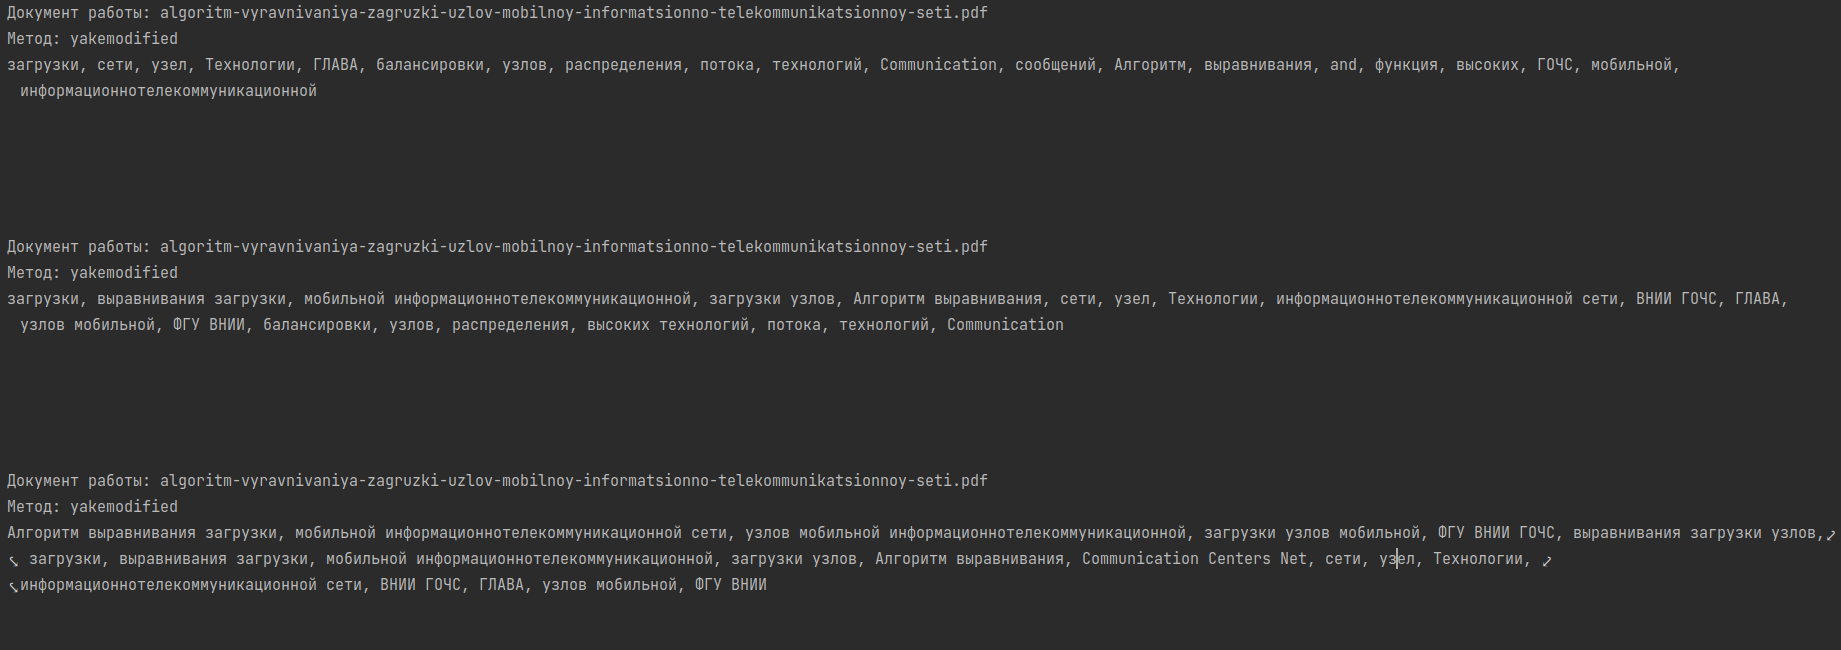
\includegraphics[width=1\linewidth]{src/img/experiment/experiment_2_4}
	\caption{Результат работы алгоритма от параметра n}
	\label{fig:experiment24}
\end{figure}
Как и предполагалось в зависимости от параметра n будут появляться многокомпонентные термины, размер которых связан с  данным параметром.
При n = 1, однокомпонентные КС, при n = 2 двухкомпонентные, при n = 3 трехкомпонентные.
Примером расширения ключевого слова является "информационнотелекоммуникационной" который преобразуется в "информационнотелекоммуникационной сети" и "мобильной информационнотелекоммуникационной" (рисунок \ref{fig:experiment24}), а затем в "мобильной информационнотелекоммуникационной сети"

\subsection{Исследование точности метода}
В рамках данного эксперимента оценивается результат работы модифицированного метода Yakе на ранее подготовленных тестовых данных, путем замера процентного пересечения ключевых слов, отмеченных авторами текста с КС полученными в результате работы метода.

Для алгоритма Yake были выставлены параметры отображенные на рисунке \ref{fig:experiment11}
\begin{figure}[!h]
	\centering
	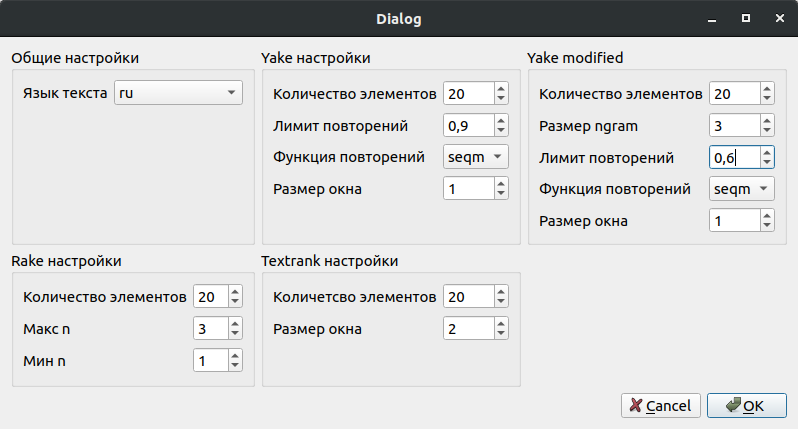
\includegraphics[width=1\linewidth]{src/img/experiment/experiment_1_1}
	\caption{Параметры модифицированного метода Yake}
	\label{fig:experiment11}
\end{figure}

На рисунке \ref{fig:experiment12} представлен результат сравнения ключевых слов предоставленных авторами документов с КС полученные путем извлечения.
В ходе данного эксперимента было установлено что процент пересечения оригинальных слов и полученных путем извлечения составляет $42\%$.
\begin{figure}[!h]
	\centering
	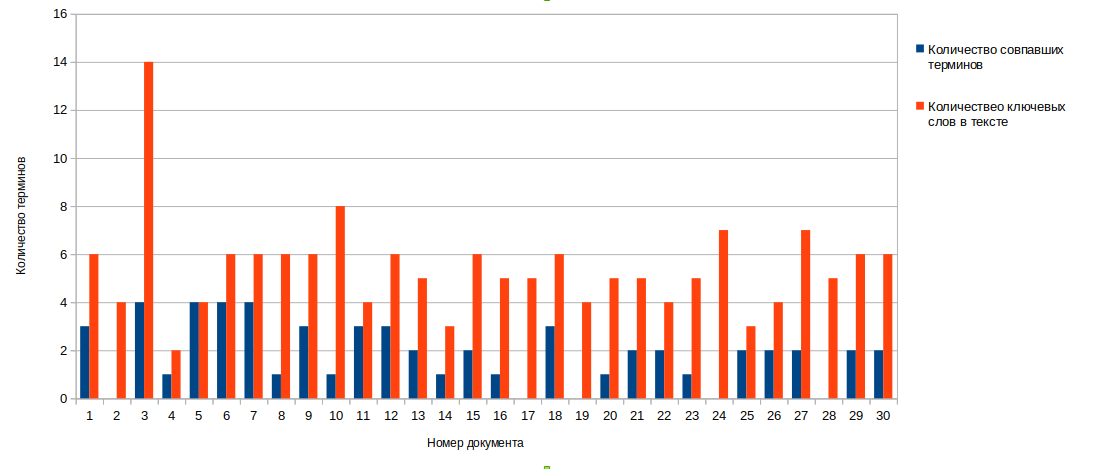
\includegraphics[width=1\linewidth]{src/img/experiment/experiment_1_2}
	\caption{Результат пересения ключевых слов}
	\label{fig:experiment12}
\end{figure}

\subsection{Исследование эффективности метода}
В процессе данного эксперимента ставится задача сравнить модифицированный метод с аналогами, способными на работу с документами на русском языке.
Для этой цели были выбраны следующие алгоритмы:
\begin{enumerate}
	\item Rake;
	\item Textrank.
\end{enumerate}
В качестве тестовых данных использовались тридцать ранее отобранных документов с ключевыми словами.
Метрикой эффективности берется процент пересечения ключевых слов полученных в результате работы алгоритмы с КС, указанных в документах авторами текстов.

Для методов были выбраны следующие настройки, отображенные на рисунке \ref{fig:experiment31}
\begin{figure}[!h]
	\centering
	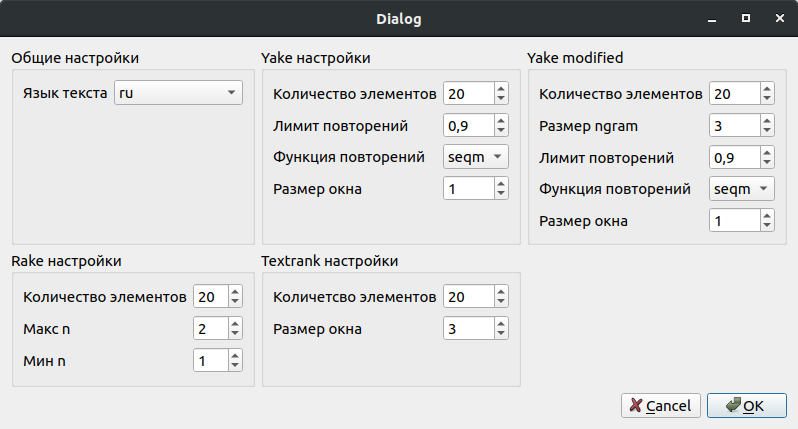
\includegraphics[width=1\linewidth]{src/img/experiment/experiment_3_1}
	\caption{Параметры методов}
	\label{fig:experiment31}
\end{figure}

Результат сравнения методов отображен на рисунке \ref{fig:experiment32}
\begin{figure}[!h]
	\centering
	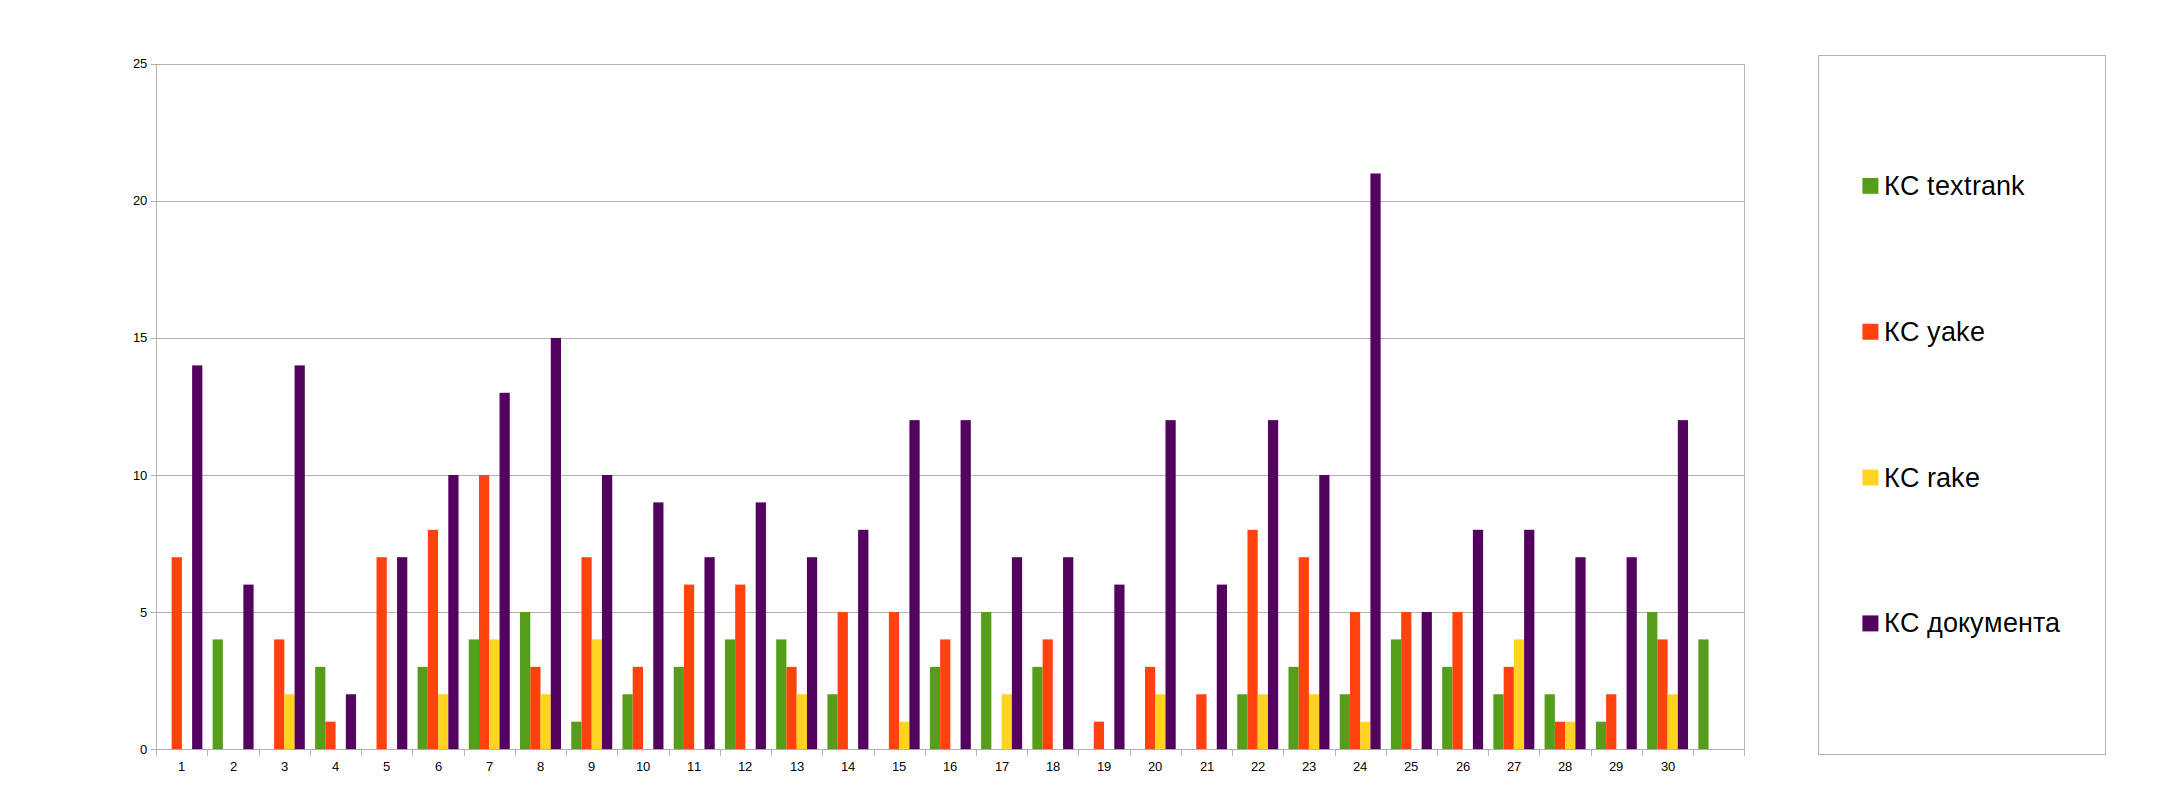
\includegraphics[width=1\linewidth]{src/img/experiment/experiment_3_2}
	\caption{}
	\label{fig:experiment32}
\end{figure}

По завершению измерений результативности были получены следующие результаты, отображенные в таблице на странице \pageref{table:experiment31}
\begin{table}[!h]
	\begin{tabular}{|c|c|c|c|}
		\hline
		& Yake (mod) & Textrank & Rake \\
		\hline
		Максимальный \% пересечения & 100\% & 71\% & 50\% \\
		\hline
		Средний \% пересечения & 42\% & 25\% & 2\% \\
		\hline
		Минимальный \% пересечения & 0\% & 0\% & \%0 \\
		\hline
	\end{tabular}
	\label{table:experiment31}
	\caption{Результат сравнения методов}
\end{table}
При сравнении результатов извлечения ключевых слов по усредненным показателям пересечения, выходит что произведенная модификация алгоритма Yake на 17\%  точнее Textrank и на 40\% метод Rake.


\subsection{Вывод}
В результате проведенной исследовательской работы над разработанным решением было установлено, что все требования, поставленные к алгоритму, соблюдены.
Метод способен на извлечение многокомпонентных ключевых слов из документов на русском языке. 
